% Options for packages loaded elsewhere
\PassOptionsToPackage{unicode}{hyperref}
\PassOptionsToPackage{hyphens}{url}
%
\documentclass[
]{article}
\usepackage{lmodern}
\usepackage{amssymb,amsmath}
\usepackage{ifxetex,ifluatex}
\ifnum 0\ifxetex 1\fi\ifluatex 1\fi=0 % if pdftex
  \usepackage[T1]{fontenc}
  \usepackage[utf8]{inputenc}
  \usepackage{textcomp} % provide euro and other symbols
\else % if luatex or xetex
  \usepackage{unicode-math}
  \defaultfontfeatures{Scale=MatchLowercase}
  \defaultfontfeatures[\rmfamily]{Ligatures=TeX,Scale=1}
\fi
% Use upquote if available, for straight quotes in verbatim environments
\IfFileExists{upquote.sty}{\usepackage{upquote}}{}
\IfFileExists{microtype.sty}{% use microtype if available
  \usepackage[]{microtype}
  \UseMicrotypeSet[protrusion]{basicmath} % disable protrusion for tt fonts
}{}
\makeatletter
\@ifundefined{KOMAClassName}{% if non-KOMA class
  \IfFileExists{parskip.sty}{%
    \usepackage{parskip}
  }{% else
    \setlength{\parindent}{0pt}
    \setlength{\parskip}{6pt plus 2pt minus 1pt}}
}{% if KOMA class
  \KOMAoptions{parskip=half}}
\makeatother
\usepackage{xcolor}
\IfFileExists{xurl.sty}{\usepackage{xurl}}{} % add URL line breaks if available
\IfFileExists{bookmark.sty}{\usepackage{bookmark}}{\usepackage{hyperref}}
\hypersetup{
  pdftitle={Assignment 3},
  pdfauthor={Group 4},
  hidelinks,
  pdfcreator={LaTeX via pandoc}}
\urlstyle{same} % disable monospaced font for URLs
\usepackage[margin=1in]{geometry}
\usepackage{color}
\usepackage{fancyvrb}
\newcommand{\VerbBar}{|}
\newcommand{\VERB}{\Verb[commandchars=\\\{\}]}
\DefineVerbatimEnvironment{Highlighting}{Verbatim}{commandchars=\\\{\}}
% Add ',fontsize=\small' for more characters per line
\usepackage{framed}
\definecolor{shadecolor}{RGB}{248,248,248}
\newenvironment{Shaded}{\begin{snugshade}}{\end{snugshade}}
\newcommand{\AlertTok}[1]{\textcolor[rgb]{0.94,0.16,0.16}{#1}}
\newcommand{\AnnotationTok}[1]{\textcolor[rgb]{0.56,0.35,0.01}{\textbf{\textit{#1}}}}
\newcommand{\AttributeTok}[1]{\textcolor[rgb]{0.77,0.63,0.00}{#1}}
\newcommand{\BaseNTok}[1]{\textcolor[rgb]{0.00,0.00,0.81}{#1}}
\newcommand{\BuiltInTok}[1]{#1}
\newcommand{\CharTok}[1]{\textcolor[rgb]{0.31,0.60,0.02}{#1}}
\newcommand{\CommentTok}[1]{\textcolor[rgb]{0.56,0.35,0.01}{\textit{#1}}}
\newcommand{\CommentVarTok}[1]{\textcolor[rgb]{0.56,0.35,0.01}{\textbf{\textit{#1}}}}
\newcommand{\ConstantTok}[1]{\textcolor[rgb]{0.00,0.00,0.00}{#1}}
\newcommand{\ControlFlowTok}[1]{\textcolor[rgb]{0.13,0.29,0.53}{\textbf{#1}}}
\newcommand{\DataTypeTok}[1]{\textcolor[rgb]{0.13,0.29,0.53}{#1}}
\newcommand{\DecValTok}[1]{\textcolor[rgb]{0.00,0.00,0.81}{#1}}
\newcommand{\DocumentationTok}[1]{\textcolor[rgb]{0.56,0.35,0.01}{\textbf{\textit{#1}}}}
\newcommand{\ErrorTok}[1]{\textcolor[rgb]{0.64,0.00,0.00}{\textbf{#1}}}
\newcommand{\ExtensionTok}[1]{#1}
\newcommand{\FloatTok}[1]{\textcolor[rgb]{0.00,0.00,0.81}{#1}}
\newcommand{\FunctionTok}[1]{\textcolor[rgb]{0.00,0.00,0.00}{#1}}
\newcommand{\ImportTok}[1]{#1}
\newcommand{\InformationTok}[1]{\textcolor[rgb]{0.56,0.35,0.01}{\textbf{\textit{#1}}}}
\newcommand{\KeywordTok}[1]{\textcolor[rgb]{0.13,0.29,0.53}{\textbf{#1}}}
\newcommand{\NormalTok}[1]{#1}
\newcommand{\OperatorTok}[1]{\textcolor[rgb]{0.81,0.36,0.00}{\textbf{#1}}}
\newcommand{\OtherTok}[1]{\textcolor[rgb]{0.56,0.35,0.01}{#1}}
\newcommand{\PreprocessorTok}[1]{\textcolor[rgb]{0.56,0.35,0.01}{\textit{#1}}}
\newcommand{\RegionMarkerTok}[1]{#1}
\newcommand{\SpecialCharTok}[1]{\textcolor[rgb]{0.00,0.00,0.00}{#1}}
\newcommand{\SpecialStringTok}[1]{\textcolor[rgb]{0.31,0.60,0.02}{#1}}
\newcommand{\StringTok}[1]{\textcolor[rgb]{0.31,0.60,0.02}{#1}}
\newcommand{\VariableTok}[1]{\textcolor[rgb]{0.00,0.00,0.00}{#1}}
\newcommand{\VerbatimStringTok}[1]{\textcolor[rgb]{0.31,0.60,0.02}{#1}}
\newcommand{\WarningTok}[1]{\textcolor[rgb]{0.56,0.35,0.01}{\textbf{\textit{#1}}}}
\usepackage{graphicx,grffile}
\makeatletter
\def\maxwidth{\ifdim\Gin@nat@width>\linewidth\linewidth\else\Gin@nat@width\fi}
\def\maxheight{\ifdim\Gin@nat@height>\textheight\textheight\else\Gin@nat@height\fi}
\makeatother
% Scale images if necessary, so that they will not overflow the page
% margins by default, and it is still possible to overwrite the defaults
% using explicit options in \includegraphics[width, height, ...]{}
\setkeys{Gin}{width=\maxwidth,height=\maxheight,keepaspectratio}
% Set default figure placement to htbp
\makeatletter
\def\fps@figure{htbp}
\makeatother
\setlength{\emergencystretch}{3em} % prevent overfull lines
\providecommand{\tightlist}{%
  \setlength{\itemsep}{0pt}\setlength{\parskip}{0pt}}
\setcounter{secnumdepth}{-\maxdimen} % remove section numbering

\title{Assignment 3}
\author{Group 4}
\date{}

\begin{document}
\maketitle

\hypertarget{instructions}{%
\section{Instructions}\label{instructions}}

Consider the stochastic process of spread of an epidemics (of COVID-19,
influenza, or other similar viruses) in a population composed by N
individuals. Assume that each individual at each time step can be in one
of the following 3 states: - S = susceptible = not infected and not
immune (then s/he can be infected) - I = infected - R = removed =
recovered and immune, or dead

Assume also that: - at each time step each susceptible individual
becomes infected with probability 0.08 - each infected individual is
removed with probability 0.6 - each removed individual returns back to
be susceptible with probability 0.1.

Represent the evolution of the epidemics as a Markov chain and write the
transition matrix.

Imagine now that the number N of individuals in the population is N =
10000.

If is it possible, find what will be the number of individuals in the
three states S,I,R in the long run, after many time steps.

\hypertarget{solution}{%
\section{Solution}\label{solution}}

\hypertarget{hypothesis-and-constraints}{%
\subsection{Hypothesis and
Constraints}\label{hypothesis-and-constraints}}

We can approach this kind of problem interpreting the system as an
oriented graph where: - nodes are the states of individuals - edges are
the transitions between a state and another

Our modeling assumption is that we consider the transitions as a process
where teh distribution of the forthcoming state \(X_{n+1}\) depends only
on the current state \(X_n\) and not on the previous ones
\(X_{n−1}, X_{n−2},...,X_1\). This implies that the conditional
probabilities of each state depend only on the state immediaely before
\$ Pr(X\_\{n+1\} = x\_\{n+1\} \textbar X\_n = x\_n )\$.

The transition that verifies at each step of the process happens with
same magnitude.

In other word it's a Stationary Process - a process where the state of
time \(t_{i+1}\), given \((t_0,...,t_n)\), depends completely and only
on the state of time \(t_{i}\).

Given all these assumptions and correspondence we can use Markov Chain
model as it fits with our assumptions an inputs.

\begin{Shaded}
\begin{Highlighting}[]
\KeywordTok{library}\NormalTok{(}\StringTok{"markovchain"}\NormalTok{)}
\end{Highlighting}
\end{Shaded}

\begin{verbatim}
## Package:  markovchain
## Version:  0.8.5-2
## Date:     2020-09-07
## BugReport: https://github.com/spedygiorgio/markovchain/issues
\end{verbatim}

\hypertarget{construction-of-inputs-and-theoretical-assumptions}{%
\subsection{Construction of Inputs and Theoretical
Assumptions}\label{construction-of-inputs-and-theoretical-assumptions}}

We have the probabilities of transit from a state to another, so we try
to group them in a single Transition Matrix.

Being a \textbf{stochastic Markov chain}: - all the elements are non
negative (from the property of \textbf{Positivity} of the probabilities
\(P(X)>=0\)) - the sum of rows and columns are equal to one (derived
from properties of \textbf{Certainty} of the probabilities
\(\sum_{i,j=1}^{n,m} x_i = 1\))

Then we can infer which are the remaining transition probabilities that
we do not have explicitly.

In particular we assume that:

\begin{itemize}
\item
  being a virus, the probability of becoming again susceptible (S) after
  being infected (I) is zero or approximately zero because of an
  Immunity factor - even if there are evidence against this assumption
  in the real world
\item
  all the individuals, at the beginning of the epidemic (\(t_0\))
  phenomenon, were susceptible (not infected and not immune) as the
  virus didn't spread yet. This characteristic can help us the derive
  the initial probability distribution \$ \mu = (\mu\_S\^{}\{(0)\},
  \mu\_I\^{}\{(0)\}, \mu\_R\^{}\{(0)\})\$
\end{itemize}

\begin{Shaded}
\begin{Highlighting}[]
\NormalTok{N <-}\StringTok{ }\DecValTok{10000} \CommentTok{# where N is the number of individuals}

\NormalTok{eipdemicsStates <-}\StringTok{ }\KeywordTok{c}\NormalTok{(}\StringTok{"S"}\NormalTok{, }\StringTok{"I"}\NormalTok{, }\StringTok{"R"}\NormalTok{)}

\CommentTok{# assuming as initial distribution}
\NormalTok{initialDistribution <-}\StringTok{ }\KeywordTok{c}\NormalTok{(}\DecValTok{1}\NormalTok{, }\DecValTok{0}\NormalTok{, }\DecValTok{0}\NormalTok{) }

\CommentTok{# we instantiate the transition matrix directly as a Markov chain data type}
\NormalTok{byRow <-}\StringTok{ }\OtherTok{TRUE}

\NormalTok{mcEpidemics <-}\StringTok{ }\KeywordTok{new}\NormalTok{(}\StringTok{"markovchain"}\NormalTok{, }
                   \DataTypeTok{states =}\NormalTok{ eipdemicsStates,}
                   \DataTypeTok{transitionMatrix =} \KeywordTok{matrix}\NormalTok{(}
                     \DataTypeTok{data =}  \KeywordTok{c}\NormalTok{(}\FloatTok{0.9}\NormalTok{, }\FloatTok{0.08}\NormalTok{, }\FloatTok{0.02}\NormalTok{,}
                               \FloatTok{0.0}\NormalTok{, }\FloatTok{0.4}\NormalTok{, }\FloatTok{0.6}\NormalTok{,}
                               \FloatTok{0.1}\NormalTok{, }\FloatTok{0.52}\NormalTok{, }\FloatTok{0.38}\NormalTok{),}
                     \DataTypeTok{byrow =}\NormalTok{ byRow,}
                     \DataTypeTok{ncol =} \DecValTok{3}\NormalTok{,}
                     \DataTypeTok{nrow =} \DecValTok{3}\NormalTok{),}
                   \DataTypeTok{name =} \StringTok{"Epidemics"}\NormalTok{)}
\CommentTok{# return}
\NormalTok{mcEpidemics}
\end{Highlighting}
\end{Shaded}

\begin{verbatim}
## Epidemics 
##  A  3 - dimensional discrete Markov Chain defined by the following states: 
##  S, I, R 
##  The transition matrix  (by rows)  is defined as follows: 
##     S    I    R
## S 0.9 0.08 0.02
## I 0.0 0.40 0.60
## R 0.1 0.52 0.38
\end{verbatim}

Where the probability of moving from state \(i\) to \(j\) in \(n\) steps
is denoted by \(p(n)ij = P r (X_n = s_j |X_0 = s_i)\)

\begin{Shaded}
\begin{Highlighting}[]
\NormalTok{mcDf <-}\StringTok{ }\KeywordTok{as}\NormalTok{(mcEpidemics, }\StringTok{"data.frame"}\NormalTok{)}
\NormalTok{mcMatrix <-}\StringTok{ }\KeywordTok{as}\NormalTok{(mcEpidemics, }\StringTok{"matrix"}\NormalTok{)}
\NormalTok{mcNew <-}\StringTok{ }\KeywordTok{as}\NormalTok{(mcDf, }\StringTok{"markovchain"}\NormalTok{)}

\CommentTok{# return}
\NormalTok{mcDf}
\end{Highlighting}
\end{Shaded}

\begin{verbatim}
##   t0 t1 prob
## 1  S  S 0.90
## 2  S  I 0.08
## 3  S  R 0.02
## 4  I  S 0.00
## 5  I  I 0.40
## 6  I  R 0.60
## 7  R  S 0.10
## 8  R  I 0.52
## 9  R  R 0.38
\end{verbatim}

\hypertarget{properties-of-the-markov-chain}{%
\subsection{Properties of the Markov
Chain}\label{properties-of-the-markov-chain}}

As we have just one transition matrix, then the Markov chain is
\textbf{time homogeneous}. In other terms,
\(Pr (X_{n+1} = sj |X_n = s_i) = Pr(X_n = s_j |X_{n−1} = s_i)\).

Furthermore, it is a \textbf{discrete} Markov Chain, because, as we're
dealing with people, talking about a person in a continuous manner does
not make sense.

It is easy to see that the chain is \textbf{irreducible} since all the
states communicate (it is made by one communicating class only).

\begin{Shaded}
\begin{Highlighting}[]
\KeywordTok{is.irreducible}\NormalTok{(mcEpidemics)}
\end{Highlighting}
\end{Shaded}

\begin{verbatim}
## [1] TRUE
\end{verbatim}

\begin{Shaded}
\begin{Highlighting}[]
\KeywordTok{plot}\NormalTok{(mcEpidemics)}
\end{Highlighting}
\end{Shaded}

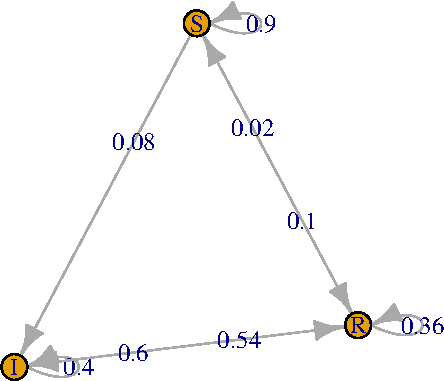
\includegraphics{assign3_group4_solution_files/figure-latex/Plot of the Graph-1.pdf}

\hypertarget{long-term-behavior}{%
\subsection{Long Term Behavior}\label{long-term-behavior}}

A periodic MC of period that, loosely speaking, means that it can only
return to itself after a fixed number of transitions \$
k\_i\textgreater1 \$ (or multiple of \(k_i\)) - else it is aperiodic.
The transition matrix is of period 1 - then it's \textbf{aperiodic}

\begin{Shaded}
\begin{Highlighting}[]
\KeywordTok{period}\NormalTok{(mcEpidemics)}
\end{Highlighting}
\end{Shaded}

\begin{verbatim}
## [1] 1
\end{verbatim}

\hypertarget{asymptotic-properties}{%
\subsection{Asymptotic Properties}\label{asymptotic-properties}}

This can help us to predict the asymptotic behavior of the system.

In fact, combining both irreducibility and aperiodicity we can state
that the system will reach any state in a finite number of steps. That a
finite state exists for this MC.

It also mean that it's distribution will settle down to a defined one, a
steady state rather than fluctuating infinitely. This distribution is
the following one:

\begin{Shaded}
\begin{Highlighting}[]
\NormalTok{steadyState <-}\StringTok{ }\KeywordTok{steadyStates}\NormalTok{(mcEpidemics)}
\NormalTok{steadyState}
\end{Highlighting}
\end{Shaded}

\begin{verbatim}
##              S         I         R
## [1,] 0.3333333 0.3333333 0.3333333
\end{verbatim}

But how many steps do we need to reach the steady state? We set up an
algorithm to calculate this - for educational purpose:

\begin{Shaded}
\begin{Highlighting}[]
\CommentTok{# asn <- initialDistribution * mcEpidemics}
\CommentTok{# }
\CommentTok{# for (i in 1:5) \{}
\CommentTok{#   if (ans == steadyState) \{}
\CommentTok{#     print(i)}
\CommentTok{#     break}
\CommentTok{#   \}}
\CommentTok{#   else \{}
\CommentTok{#     ans <- initialDistribution * ans}
\CommentTok{#   \}}
\CommentTok{# \}}
\end{Highlighting}
\end{Shaded}

\hypertarget{number-of-individuals-asymptotically-distributed}{%
\subsection{Number of Individuals Asymptotically
Distributed}\label{number-of-individuals-asymptotically-distributed}}

We simulate the trend of the MC after many steps

\begin{Shaded}
\begin{Highlighting}[]
\KeywordTok{library}\NormalTok{(ggplot2)}

\NormalTok{initState <-}\StringTok{ }\NormalTok{initialDistribution}
\NormalTok{manySteps <-}\StringTok{ }\DecValTok{100}

\CommentTok{# Instantiate probability vectors}
\NormalTok{P_S <-}\StringTok{ }\KeywordTok{c}\NormalTok{()}
\NormalTok{P_I <-}\StringTok{ }\KeywordTok{c}\NormalTok{()}
\NormalTok{P_R <-}\StringTok{ }\KeywordTok{c}\NormalTok{()}

\CommentTok{# Calculate probabilities for 100 steps.}
\ControlFlowTok{for}\NormalTok{(k }\ControlFlowTok{in} \DecValTok{1}\OperatorTok{:}\DecValTok{100}\NormalTok{)\{}
\NormalTok{  nsteps <-}\StringTok{ }\NormalTok{initState }\OperatorTok{*}\StringTok{ }\NormalTok{(mcEpidemics }\OperatorTok{^}\StringTok{ }\NormalTok{k)}
\NormalTok{  P_S[k] <-}\StringTok{ }\NormalTok{nsteps[}\DecValTok{1}\NormalTok{,}\DecValTok{1}\NormalTok{]}
\NormalTok{  P_I[k] <-}\StringTok{ }\NormalTok{nsteps[}\DecValTok{1}\NormalTok{,}\DecValTok{2}\NormalTok{]}
\NormalTok{  P_R[k] <-}\StringTok{ }\NormalTok{nsteps[}\DecValTok{1}\NormalTok{,}\DecValTok{3}\NormalTok{]}
\NormalTok{\}}

\CommentTok{# Make dataframes and merge them}

\CommentTok{# S}
\NormalTok{P_S <-}\StringTok{ }\KeywordTok{as.data.frame}\NormalTok{(P_S)}
\NormalTok{P_S}\OperatorTok{$}\NormalTok{Group <-}\StringTok{ 'Susceptible'}
\NormalTok{P_S}\OperatorTok{$}\NormalTok{Iter <-}\StringTok{ }\DecValTok{1}\OperatorTok{:}\NormalTok{manySteps}
\KeywordTok{names}\NormalTok{(P_S)[}\DecValTok{1}\NormalTok{] <-}\StringTok{ 'Value'}

\CommentTok{# I}
\NormalTok{P_I <-}\StringTok{ }\KeywordTok{as.data.frame}\NormalTok{(P_I)}
\NormalTok{P_I}\OperatorTok{$}\NormalTok{Group <-}\StringTok{ 'Infected'}
\NormalTok{P_I}\OperatorTok{$}\NormalTok{Iter <-}\StringTok{ }\DecValTok{1}\OperatorTok{:}\NormalTok{manySteps}
\KeywordTok{names}\NormalTok{(P_I)[}\DecValTok{1}\NormalTok{] <-}\StringTok{ 'Value'}

\CommentTok{# R}
\NormalTok{P_R <-}\StringTok{ }\KeywordTok{as.data.frame}\NormalTok{(P_R)}
\NormalTok{P_R}\OperatorTok{$}\NormalTok{Group <-}\StringTok{ 'Removed'}
\NormalTok{P_R}\OperatorTok{$}\NormalTok{Iter <-}\StringTok{ }\DecValTok{1}\OperatorTok{:}\NormalTok{manySteps}
\KeywordTok{names}\NormalTok{(P_R)[}\DecValTok{1}\NormalTok{] <-}\StringTok{ 'Value'}

\CommentTok{# steps}
\NormalTok{steps <-}\StringTok{ }\KeywordTok{rbind}\NormalTok{(P_S,P_I,P_R)}

\CommentTok{# Plot the probabilities using ggplot}
\KeywordTok{ggplot}\NormalTok{(steps, }\KeywordTok{aes}\NormalTok{(}\DataTypeTok{x =}\NormalTok{ Iter, }\DataTypeTok{y =}\NormalTok{ Value, }\DataTypeTok{col =}\NormalTok{ Group))}\OperatorTok{+}
\StringTok{  }\KeywordTok{geom_line}\NormalTok{() }\OperatorTok{+}
\StringTok{  }\KeywordTok{xlab}\NormalTok{(}\StringTok{'Chain Step'}\NormalTok{) }\OperatorTok{+}
\StringTok{  }\KeywordTok{ylab}\NormalTok{(}\StringTok{'Probability'}\NormalTok{) }\OperatorTok{+}
\StringTok{  }\KeywordTok{ggtitle}\NormalTok{(}\KeywordTok{paste0}\NormalTok{(manySteps,}\StringTok{' Steps Chain Probability Prediction'}\NormalTok{, }\DataTypeTok{collapse =} \OtherTok{NULL}\NormalTok{)) }\OperatorTok{+}\StringTok{ }
\StringTok{  }\KeywordTok{theme}\NormalTok{(}\DataTypeTok{plot.title =} \KeywordTok{element_text}\NormalTok{(}\DataTypeTok{hjust =} \FloatTok{0.5}\NormalTok{))}
\end{Highlighting}
\end{Shaded}

\includegraphics{assign3_group4_solution_files/figure-latex/Asymptotical Distribution of MC-1.pdf}

\hypertarget{conclusion}{%
\section{Conclusion}\label{conclusion}}

The number of individuals in each state is calculated through the
\textbf{expected value} - probability of being in a particular state
times the total number of individuals

\$ E(X)=P(s\_i)*N \$

\begin{Shaded}
\begin{Highlighting}[]
\NormalTok{nS_i <-}\StringTok{ }\KeywordTok{round}\NormalTok{(steadyState }\OperatorTok{*}\StringTok{ }\NormalTok{N)}
\NormalTok{nS_i}
\end{Highlighting}
\end{Shaded}

\begin{verbatim}
##         S    I    R
## [1,] 3333 3333 3333
\end{verbatim}

\end{document}
